% !TEX root = thesis.tex
\documentclass[thesis.tex]{subfiles} 
\begin{document}

\chapter{Demo applications}
% \todo{Re-enable the graphics. LaTeXTools don't seem to work with it}
\label{chap:demo}
This chapter describes two applications utilizing Comb to make a case for
its relevance in the web development area and to illustrate the internal
workings of Comb.
The first application shows an actual use case of Comb and highlights its
strengths by comparison with jQuery. To that end the applications has been
developed in four different versions.

The second application demonstrates the internal workings of Comb by using Combs
ability to analyze templates and extract the original dataset fed into the
template engine. The structure of the dataset will then be used to build a form
to allow changing its values.

\section{Movie Database \#2}
In the exploratory prototype (chapter \ref{chap:prototype}) we created a
Movie Database to organize information about the cast, year of release as well
as the plot and synopsis of a movie. We reimplemented the same application
in much the same way.

We use chaplin\footnote{See appendix \ref{app:chaplin}} to structure our
application on the client-side, while a PHP REST framework together with
php-activerecord function as a communication layer to the MySQL database for the
client.
The client code is written in CoffeeScript\footnote{See
section \ref{sec:coffeescript}}.

The document root of the web application presents the user with two links to
the same Movie Database implemented in two slightly different ways.
The first link leads to an implementation using the CSS and HTML structure from
our exploratory prototype.
The second link leads to a different version of the application where we use the
Twitter Bootstrap\footnote{See appendix \ref{app:bootstrap}} library to style
the interface, instead of the original CSS and HTML.

In both implementations, Movies can be browsed, created and edited. Examples of
both versions can be seen in figures \ref{fig:moviedb-prototype} and
\ref{fig:moviedb-bootstrap}

\begin{figure}
	\centering
	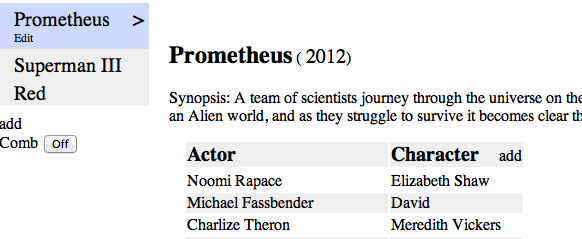
\includegraphics[max width=\linewidth]{graphics/moviedb-prototype}
	\caption{Original prototype implementation of the Movie Database application}
	\label{fig:moviedb-prototype}
\end{figure}

\begin{figure}
	\centering
	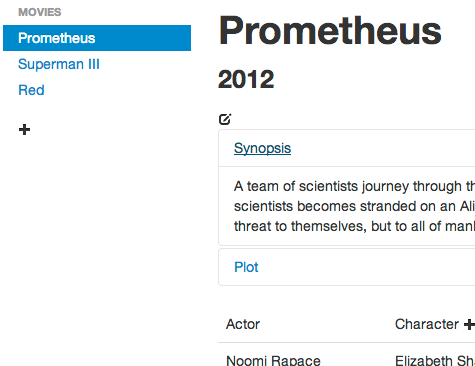
\includegraphics[max width=\linewidth]{graphics/moviedb-bootstrap}
	\caption{Bootstrap implementation of the Movie Database application}
	\label{fig:moviedb-bootstrap}
\end{figure}

\subsection{Architecture}
The HTML page is built with server-side mustache templates. Interactivity is
then added once the client application has started.
We use chaplin views to split sections of the web application into the following
manageable parts:

\begin{itemize}
\item \emph{Movies}: A ViewCollection representing the list of movies available
                     in the database
\item \emph{Movie}: A View managing the DOM subtree of a single movie.
\item \emph{Cast}: A ViewCollection containing all roles in a movie.
\item \emph{Role}: A single Role in the Cast, this is the relationship
                   connecting a movie and an actor.
\item \emph{Actor}: An actor playing a role
\end{itemize}

When initializing the client application, we bind DOM subtrees from the HTML
created by the server to the corresponding Views. Each view is responsible for
retrieving values from the DOM to populate the Model it is holding, while also
initializing subviews that belong to it.
In the case of the Movies CollectionView, we iterate over the list of movies and
instantiate a new Movie View for each list element we encounter.
Once a Movie View has been created we access the Model the View has populated
and push it onto our collection of movies. The corresponding code can be seen in
figure \ref{fig:movies-iter}.
\begin{figure}
	\centering
	\begin{lstlisting}
@$list = @$ @listSelector
for el in @$list.children()
	view = new MovieView {el}
	@subview "itemView:#{view.model.cid}", view
	# Silent push, we do not want chaplin to create a new view
	@collection.push view.model, silent: true
	\end{lstlisting}
	\caption{Initializing Movie Views}
	\label{fig:movies-iter}
\end{figure}

Once a View has populated its Model, it binds event handlers to any buttons
in the interface it should respond to when clicked.

\subsection{Retrieving DOM values}
The original version of the Movie Database from our exploratory prototype comes
in two flavors: jQuery and Comb.
These flavors refer to the strategy we use in a View to retrieve values from the
DOM and populate our Models with. We can switch between the strategies by
clicking on the button On/Off below the list of Movies.

In the jQuery strategy we use CSS selectors and jQuery
accessors\footnote{\inline{.attr('name') or .text()}} to pinpoint values in the
DOM.
Once a value is retrieved, we may also need to strip some of the parts that do
not belong to the actual value present in the database.
In figure \ref{fig:movie-jquery-prototype} we retrieve all the
values of a Movie and add them to the Movie Model.
\begin{figure}
	\centering
	\begin{lstlisting}
@model.set 'id', (@$('>details').attr 'id').substring 6
@model.set 'title', @$('summary.title').text()
@model.set 'year', @$('span.year').text()
@model.set 'synopsis', @$('summary.synopsis span').text()
@model.set 'plot', @$('details.plot p').text()
	\end{lstlisting}
	\caption{Using jQuery, we populate a Model by using selectors matching the
	template of the exploratory prototype}
	\label{fig:movie-jquery-prototype}
\end{figure}

Figure \ref{fig:movie-comb-prototype} shows the same procedure, only here we
use Comb to retrieve those values. We can clearly see that there are no
references to the structure of the template used, instead we use the exact same
names the to set model properties and access values in the dataset.
This is no coincidence, the properties of our client-side Movie Model and
those of the server-side Movie Model are the same. Therefore we must also use
them when creating our templates, which leaves us with a dataset, that mirrors
its server-side counterpart.
\begin{figure}
	\centering
	\begin{lstlisting}
@model.set 'id', @data.id.value
@model.set 'title', @data.title.value
@model.set 'year', @data.year.value
@model.set 'synopsis', @data.synopsis.value
@model.set 'plot', @data.plot.value
	\end{lstlisting}
	\caption{To populate a Model with Comb, we access the values in the dataset,
	by the names the matching Model properties has on the server.}
	\label{fig:movie-comb-prototype}
\end{figure}

\subsection{Changing templates}
\label{sec:changing-templates}
The independence from the template structure in our Comb strategy is exemplified
by our second implementation using the Bootstrap library. This version also
exists in both a jQuery and Comb flavor.

The structure of the HTML is quite different from our original implementation,
because Bootstrap requires the developer to set up his layout in a grid
system\footnote{\url{http://twitter.github.com/bootstrap/scaffolding.html\#gridSystem}}.
To expand the synopsis and plot of a movie we use the ``accordion''
widget\footnote{\url{http://twitter.github.com/bootstrap/javascript.html\#collapse}}.
This is a departure from our original layout where the native HTML5 elements
\inline{details} and \inline{summary} were used.

In figure \ref{fig:movie-jquery-bootstrap} we can see how the selectors when
using the jQuery strategy for retrieving DOM values have changed.
\begin{figure}
	\centering
	\begin{lstlisting}
@model.set 'id', (@$('>div').attr 'id').substring 6
@model.set 'title', @$('h1').text()
@model.set 'year', @$('h3').text()
@model.set 'synopsis', @$("#plot-#{@model.id} div").text()
@model.set 'plot', @$("#synopsis-#{@model.id} div").text()
	\end{lstlisting}
	\caption{The jQuery selectors used to extract values from the rendered
	template have all changed when compared with the previous selectors in
	figure \ref{fig:movie-jquery-prototype}}
	\label{fig:movie-jquery-bootstrap}
\end{figure}
Contrasting this with the Comb strategy shown in figure \ref{fig:movie-comb-bootstrap}
leaves us with a clear picture of the robustness Comb has with respect to
retrieving values from the DOM.
The code in figure \ref{fig:movie-comb-prototype} and
\ref{fig:movie-comb-bootstrap} is exactly the same.
\begin{figure}
	\centering
	\begin{lstlisting}
@model.set 'id', @data.id.value
@model.set 'title', @data.title.value
@model.set 'year', @data.year.value
@model.set 'synopsis', @data.synopsis.value
@model.set 'plot', @data.plot.value
	\end{lstlisting}
	\caption{The data extraction code utilizing Comb needed no modifications}
	\label{fig:movie-comb-bootstrap}
\end{figure}



\section{Template Editor}
The Template Editor is an application with which we can explore how Comb
functions.
It also serves as a tool for testing Comb itself.
We present the user with an interface where templates can be loaded from the
navigation bar at the top of the page. The templates all originate from our
Movie Database application. Figure \ref{fig:template-selection} shows the
navigation bar with the template selection menu open.
\begin{figure}
	\centering
	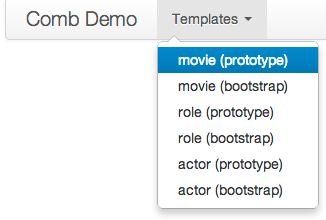
\includegraphics[max width=\linewidth]{graphics/template-selection}
	\caption{The template selection menu from the editor application}
	\label{fig:template-selection}
\end{figure}
Upon selecting a template, the application loads the template and the Comb file
using require.js (\ref{sec:requirejs}).
The template is then rendered\footnote{We use the client-side mustache.js
template engine to render templates directly in the browser.} with no initial
dataset and the results are displayed in the right view port.
Beneath it the template source code is also shown verbatim.

In the left view port a form with various buttons and input fields appears once
the template has been rendered. In figure \ref{fig:editor-form} we can see how
this form can be used to control all aspects of the dataset that is fed into
the template rendering engine.
\begin{figure}
	\centering
	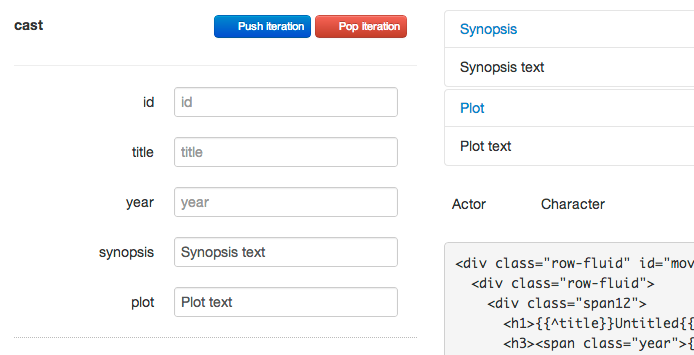
\includegraphics[max width=\linewidth]{graphics/editor-form}
	\caption{Editing the dataset for a template with a form}
	\label{fig:editor-form}
\end{figure}

As such, the application itself is rather uninteresting. The more interesting
part is the underlying architecture.

\subsection{Generating the form}
To generate the form in the left view port, we transform the dataset retrieved
from the rendered template in the left view port into a structure that fits the
form template (figure \ref{fig:mustache.mustache}) we have written in mustache
as well.
\begin{figure}
	\centering
	\lstinputlisting[language=HTML]{../Comb/Editor/app/scripts/templates/mustache.mustache}
	\caption{The file \inline{mustache.mustache}. A mustache template intended for viewing values retrieved by comb.}
	\label{fig:mustache.mustache}
\end{figure}

This template uses sections and partials to recursively iterate over the
transformed data structure.
Sections from the rendered template are displayed as a headline and two adjacent
buttons.
Variables become input fields or text areas depending on whether they are
escaped.
Partials are unfortunately not supported.

\subsection{Parsing the form}
So far we only have a form which displays the dataset values of a template that
was rendered with an empty dataset.
Since this form was rendered with mustache, we can now make it interactive by
parsing it with Comb. The buttons in the ``section'' section have
\inline{data-target} attributes so that we may bind click event listeners to
them, by using the parent nodes of the ``name'' variables. We can listen
for changes on the input fields for the escaped variables and text areas for the
unescaped variables in much the same way.

\subsection{Loopbacking Comb}
\label{sec:loopbacking}
The fields in our form have corresponding entries in the dataset passed to
the template we loaded in the beginning.
Note that although we passed an empty dataset to mustache, Comb will return
section values as empty lists (see section \ref{sec:if-else}) and
variable values as empty strings (see appendix \ref{app:mustache-vars}).
By binding event listeners to our fields we can update the original dataset
correspondingly. Changes in input fields and text areas trigger a call to the
\inline{update(text)} function on the original dataset and update the text in the
right view port.

Pushing the ``push'' button on a section appends a new entry to the array of the
original dataset, while the ``pop'' button removes the last entry from said array.
When we modify the amount of iterations in an array, we re-render the loaded
template\footnote{Section \ref{sec:update-dom} explains this necessity
in more detail.}.
\end{document}
